
%%%%%%%%%%
\subsection{Principe de détection}
\label{sec:detection_principle}

Nous nous concentrerons dans ce chapitre sur les détecteurs d'ondes gravitationnelles actuels qui reposent sur des techniques d'interférométrie laser.
Ils sont basés sur la comparaison de deux distances orthogonales de l'espace. Ces distances sont délimitées par des masses libres qui sont les miroirs d'un interféromètre de Michelson, interféromètre qui nous permet de comparer ces distances.

Dans un interféromètre, un faisceau laser est scindé en deux et envoyé vers les miroirs.
Les deux faisceaux sont réfléchis, se recombinent et le faisceau résultant est analysé par un photodétecteur.
Un schéma simple est donné en figure \ref{fig:michelson}.
Pour optimiser la sensibilité, cette recombinaison des faisceaux est choisie de sorte à ce qu'ils interfèrent de manière quasi-destructive et qu'il n'y ait donc presque aucune lumière en sortie de l'interféromètre.
On parle alors de configuration ``franges sombres''.
Le phénomène d'interférence, et donc la quantité de lumière qui peut être transmise en sortie de l'interféromètre, dépend de la différence de phase des faisceaux recombinés.
Cette différence de phase dépend à son tour directement de la difference des chemins optiques parcourus par chaque faisceau.
C'est ce concept qui est exploité pour la détection d'ondes gravitationnelles.
Pour un interféromètre dont la longueur des bras est fixée et dont les sources de bruits sont sous contrôle, la configuration de franges sombres est maintenue.

Considérons maintenant le passage d'une onde gravitationnelle au travers de cet interféromètre, avec une direction de propagation colinéaire à l'un des bras de l'interféromètre.
Ce bras va être aveugle au passage de l'onde car cette dernière n'a d'effets que le long des directions orthogonales à sa direction de propagation.
En revanche, ce n'est pas le cas pour l'autre bras de l'interféromètre.
Ainsi, la distance propre entre la séparatrice (Beam Splitter, BS) et le miroir de ce bras va osciller à cause du passage de l'onde.
Le chemin optique parcouru par le laser va donc être modifié, ce qui va causer un décalage dans la différence de phase des deux faisceaux.
Le passage de l'onde va ainsi modifier la configuration de franges sombres.
Une photodiode sensible permet de détecter cette variation et donc d'identifier le passage de l'onde gravitationnelle.

%
\begin{figure}
  \centering
  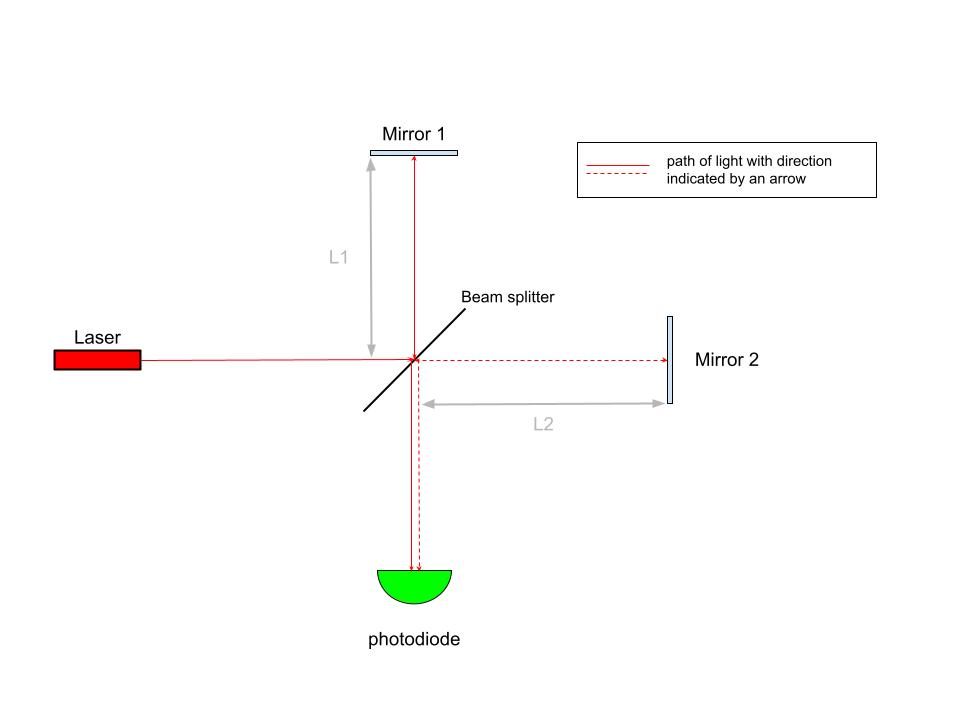
\includegraphics[width=0.8\linewidth]{sectionDetection/michelson.jpg}
  \caption{Schéma d'un interféromètre de Michelson}
  \label{fig:michelson}
\end{figure}


%%%%%%%%%%
\subsection{Description des détecteurs}
\label{sec:detector}

Les détecteurs LIGO et Virgo sont bien plus complexes qu'un interféromètre de Michelson usuel.
La quantité mesurée est appelée ``contrainte'' ou ``\textit{detector strain}''.
Elle est calculée à partir de la variation de longueur d'un bras par
\begin{equation}
  h = \frac{\Delta L}{L_0}
\end{equation}
Où $\Delta L = L_1-L_2$ est la différence de longueur entre les deux bras de l'interféromètre et $L_0 = \textrm{\SI{3}{km}} (\textrm{\SI{4}{km}})$ pour Virgo (LIGOs) est la longueur des bras au repos.
Cette contrainte est sans dimension par construction et varie avec le temps.
Elle est communément appellée ``h de t'' et notée $h(t)$.

Une schématisation de la disposition optique de Virgo pour la période d'observation O3 est présentée en figure \ref{fig:virgo_layout}.
Les détails de l'interféromètre peuvent être trouvés dans \cite{advanced_virgo,virgo_tech_report,virgo_phase2_tech_report} et les divers papiers référencés dans ce chapitre.
Nous n'allons ici qu'en présenter les parties principales afin de décrire la figure \ref{fig:virgo_layout}.
Le laser permet de délivrer un faisceau très stable.
Des modulateurs électro-optique (\textit{Electro-Optic Modulator}, EOM) sont placés après celui-ci pour créer des fréquences supplémentaires utilisées pour assurer le fonctionnement du détecteur.
Des cavités Fabry-Pérot sont présente dans chaque bras de l'interféromètre entre les ``\textit{West/North input mirrors}'' (WI/NI) et ``\textit{West/North end mirrors}'' (WE/NE).
Le faisceau, réfléchi de nombreuses fois dans ces cavités, parcours alors un chemin optique bien plus grand que la longueur des bras.
Les miroirs de 40 kg sont faits de silice fondue à faible absorption. Leurs surfaces sont recouvertes d’empilements de couche minces assurant leur propriété réfléchissante, ou anti-réfléchissante. Ils sont suspendus à une chaine de filtre mécaniques, fonctionnant dans les six degrés de libertés, assurant leur isolation des mouvements du sol pour des fréquences supérieur à quelques Hz.
Un miroir de recyclage de puissance (\textit{Power Recycling mirror}, PR) est utilisé pour réinjecter dans l’interféromètre la puissance qu’il réfléchit et augmenter de plus d’un ordre de grandeur la puissance des faisceaux circulant dans l’interféromètre.
Cela permet de réduire l'incertitude liée au bruit quantique en sortie du détecteur.
Un miroir de recyclage du signal (\textit{Signal Recycling mirror}, SR) permet également d'atteindre une meilleure sensibilité \cite{recycling1,recycling2}.
Des fractions des faisceaux sont prélevés à différents endroits de l’interféromètre pour fournir des signaux permettant d’assurer le contrôle continu du positionnement des différents éléments de l’interféromètre.
Des nettoyeurs de modes sont placés en entrée et sortie du détecteur et sont notés IMC/OMC pour \textit{Input/Output Mode Cleaner}.
Ils assurent la qualité du faisceau laser en entrée et sortie de l'interféromètre.
La photodiode B1 est placée à la sortie du détecteur pour collecter le signal contenant l'information onde gravitationelle.
L'utilisation d'une source de ``\textit{squeezed light}'' \cite{squeezer}, injectée dans l'interféromètre, permet de réduire le bruit quantique lié au comptage des photons.
La plupart de ces composants sont placés dans le vide.
%
\begin{figure}[H]
  \centering
  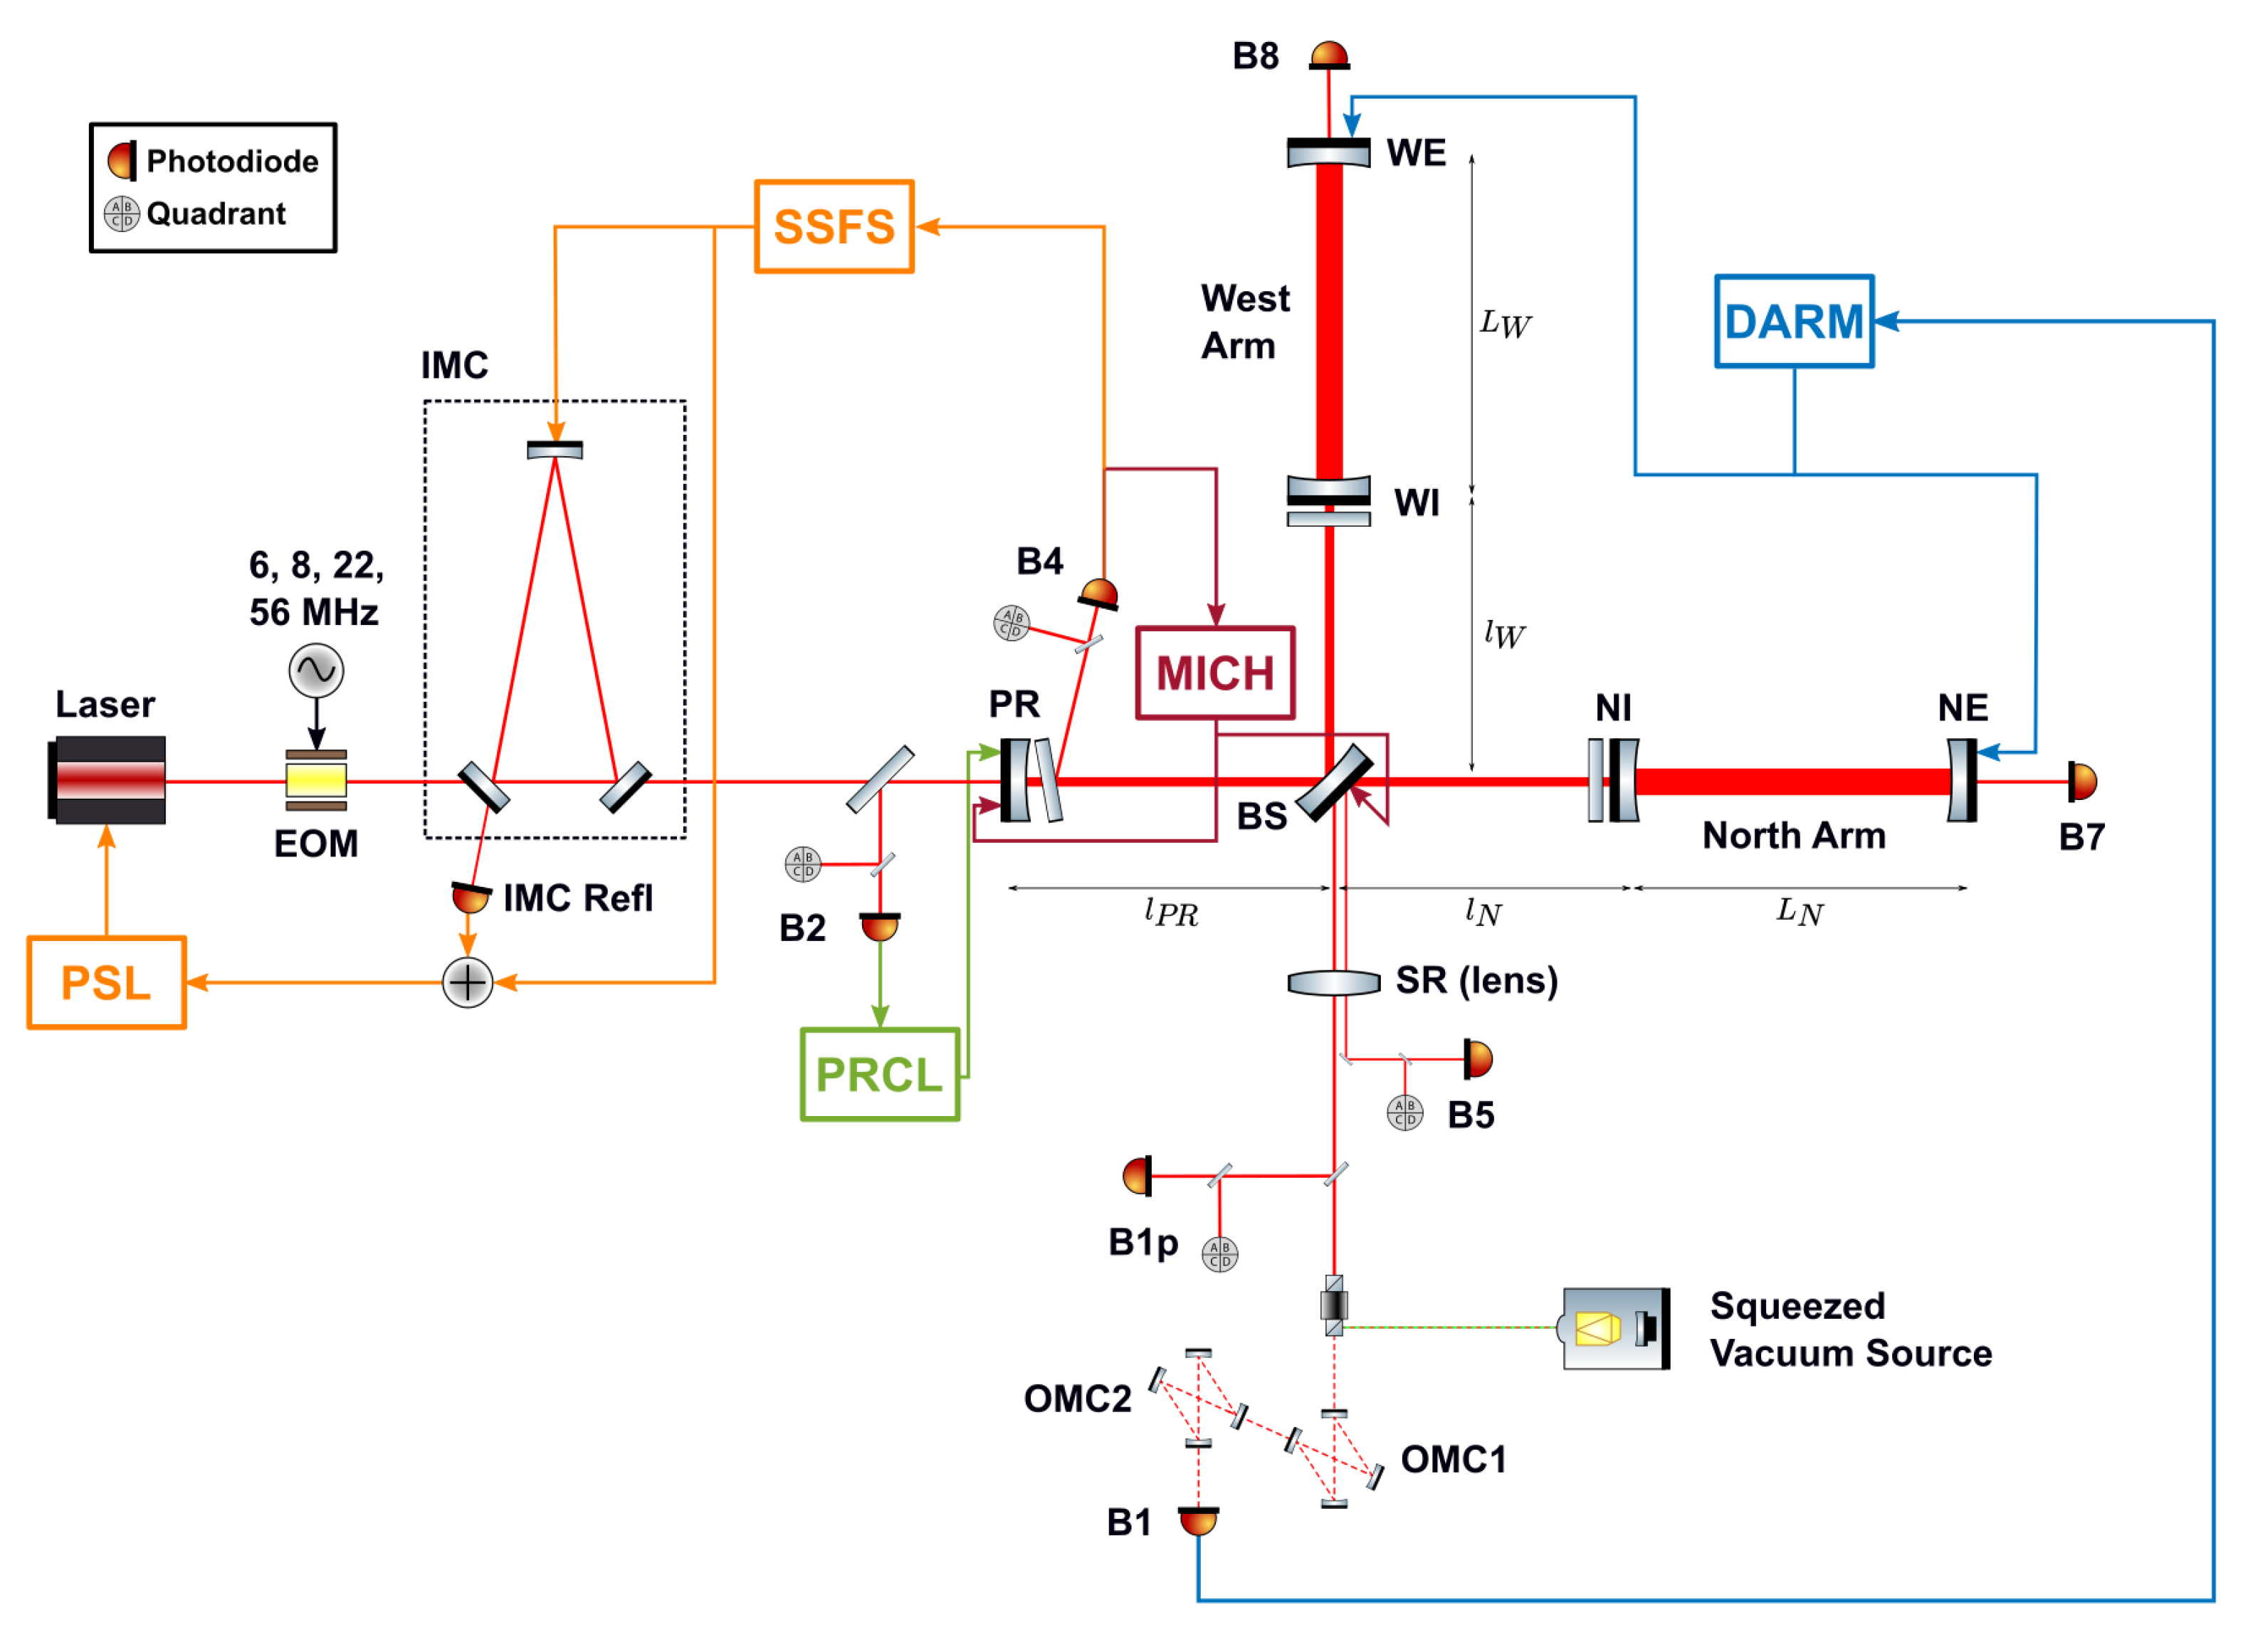
\includegraphics[width=\linewidth]{sectionDetection/virgo_layout.png}
  \caption{Dispositif optique de Virgo durant O3 provenant de \cite{virgo_layout} décrit en partie dans le texte. MICH, PRCL, CARMN et DARM sont les degrés de libertés longitudinaux charactéristiques du détecteur. Plus de détails peuvent être trouvés dans la référence.}
  \label{fig:virgo_layout}
\end{figure}
%

Des techniques de calibration ont été développées pour obtenir une mesure précise de $h(t)$:
\begin{itemize}
\item Le calibrateur photonique \cite{pcal} (PCal) utilise la modulation de la pression de radiation d'un laser pour induire un déplacement des miroirs de fin.
  Il s'agissait de la méthode de calibration de référence durant O3.
\item Le calibrateur newtonien \cite{ncal1,ncal2} (NCal) est une nouvelle technique développée pour le détecteur Virgo à Annecy puis Strasbourg.
  Le principe de cette méthode est d'induire un déplacement du miroir de fin à l'aide d'un champ gravitationnel variable, produit par des masses en rotation.
  Cette technique a, entre autre, l'avantage de ne pas nécessiter de fenêtre d'accès au miroir puisque la force gravitationnelle agit à travers la matière.
\end{itemize}
La référence \cite{strain_reconstruction} donne une vue d'ensemble de la calibration et de la reconstruction de $h(t)$ pour Virgo durant O3.


\subsubsection{Réponse d'un détecteur d'ondes gravitationnelles}

La réponse d'un détecteur à une onde gravitationnelle peut être modélisée par son diagramme d'antenne.
Cette réponse est une fonction de la direction de propagation de l'onde par rapport à l'orientation du détecteur telle que
\begin{equation}
  h = F_+ h_+ + F_\times h_\times
\end{equation}
où \cite{antenna_patterns}
\begin{align}
  F_+ &= -\frac{1}{2}(1+\cos^2\theta) \cos 2\phi \cos 2\psi - \cos \theta \sin 2\phi \sin 2 \psi\\
  F_\times &= \frac{1}{2}(1+\cos^2\theta) \cos 2\phi \sin 2\psi - \cos \theta \sin 2\phi \cos 2 \psi
\end{align}
sont les réponses d'antennes du détecteur aux polarisations ``plus'' et ``croix'' respectivement.
$\theta$ et $\phi$ sont les angles de position dans le ciel de la source des ondes et $\psi$ est l'ange de polarisation.
La figure \ref{fig:antenna_pattern} montre ces réponses pour un angle de polarisation de 0.
On remarque que le cas optimal pour une détection est lorsque l'onde se propage selon une direction orthogonale aux deux bras de l'interféromètre.
%
\begin{figure}
  \centering
  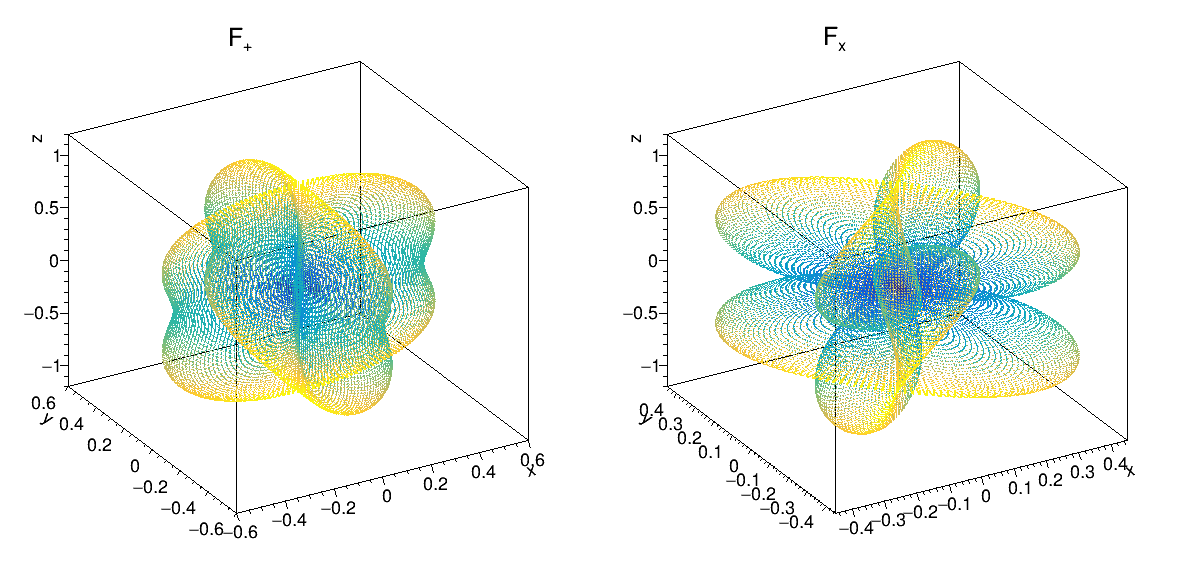
\includegraphics[width=\linewidth]{sectionDetection/antenna.png}
  \caption{Diagramme d'antenne d'un détecteur aux polarisations plus et croix.}
  \label{fig:antenna_pattern}
\end{figure}
%

La forte sensibilité des détecteurs fait qu'ils sont facilement pollués par de nombreuses sources de bruit.
La sensibilité d'un détecteur est caractérisée par la densité spectrale de puissance (\textit{Power Spectral Density}, PSD) de son bruit.
Les figures \ref{fig:ligo_sensitivity} et \ref{fig:virgo_sensitivity} montrent les contributions de différentes sources de bruit à l'amplitude de densité spectrale (\textit{Amplitude Spectral Density}, ASD) des détecteurs.


\subsubsection{Horizon et \textit{range} d'un détecteur d'ondes gravitationnelles}

Différentes quantités sont utilisées pour quantifier la sensibilité des détecteurs avec une unique valeur \cite{findchirp,distances,one_ifo}.

La distance d'horizon est définie pour un type de source et un seuil de ratio signal-sur-bruit $\rho$ (\textit{Signal-to-Noise Ratio}, SNR détaillé en section \ref{section:mbta}).
Il s'agit de la distance effective (eq. \ref{eq:effective_distance}) pour laquelle ce type de source serait détecté avec un SNR attendu de $\rho$ pour l'orientation optimale.
En d'autres termes l'horizon est la distance maximale à laquelle il est possible de détecter cette source avec le seuil donné.
L'horizon est donné par \cite{findchirp} (Appendix D)
\begin{equation}
  D_{\textrm{horizon}} = \frac{1}{\rho} \frac{(GM_c)^{5/6}}{\pi^{2/3}c^{3/2}} \frac{\msun^{5/3}}{\textrm{\SI{1}{Mpc}}} \sqrt{\left(\frac{5}{6}\right) \int_{0}^{\infty}\frac{f^{-7/3}}{S_n(f)}df}
  \label{eq:horizon}
\end{equation}
où $S_n(f)$ est la PSD du détecteur.
En pratique l'intégration est faite en commençant à $f_{\textrm{low}}$, la fréquence à laquelle la bande sensible du détecteur commence, et $f_{\textrm{ISCO}}$ la fréquence de la binaire à sa dernière orbite circulaire (dite ISCO ou encore LSO).
Cette fréquence est définie à l'ordre newtonien par
\begin{equation}
  f_{\textrm{ISCO}} = \frac{c^3}{6\sqrt{6}\pi G M_{\textrm{tot}}}
  \label{eq:f_isco}
\end{equation}
L'horizon est typiquement calculé pour un système BNS de $1.4+1.4$ \msun et un seuil de SNR $\rho=8$.

Le volume comobile redshifté $V_z$  est exprimé par unité de temps \cite{distances} et est défini par:
\begin{equation}
  V_z = \frac{ \int_{D<D_{\textrm{horizon}}} \frac{D^2}{1+z(D)} dD \hspace{1pt} d\Omega \hspace{2pt} \sin i \hspace{2pt} di \hspace{2pt} d\psi}{\int \sin i \hspace{2pt} di \hspace{2pt} d\psi}
\end{equation}
où $D$ est la distance comobile à la source, $\Omega$ est l'angle solide dans le ciel, $i$ est l'inclinaison du système binaire et $\psi$ est l'orientation de la source.

Le volume $V_z$ multiplié par le temps effectif d'observation est appelé ``volume-temps'' (VT).
Pour des évènements de type CBC, les sources des ondes gravitationnelles sont siutées à de très grandes distances, bien au-delà de l'échelle de notre galaxie.
Ainsi, la distribution de ces sources peut être considérée comme isotrope.
Pour une population de $N_{\textrm{source}}$ sources distribuées isotropement dans une sphère de rayon $D_{\textrm{horizon}}$, seul un petit nombre $N_{\textrm{det}}$ d'entre elles sera détectable car elles vérifieront $D_{\textrm{eff}}<D_{\textrm{horizon}}$.
Un volume plus grand augmente donc le nombre de sources détectables.
Le nombre de détections est proportionnel au VT.

On utilise plus communément la portée du détecteur ou ``\textit{range}'' pour se référer à la sensibilité des détecteurs.
La portée est définie comme le rayon d'une sphère de volume $V_z$:
\begin{equation}
  \frac{4}{3} \pi \times \textrm{range}^3 = V_z
\end{equation}
L'horizon étant calculé pour un type de source et un seuil de SNR donné, c'est également le cas pour la portée du détecteur.
Comme pour $V_z$, il est typiquement calculé pour un système BNS de $1.4+1.4$ \msun et un seuil de SNR de 8.
On parle alors de ``portée BNS'' ou ``\textit{BNS range}''.
Une comparaison des sensibilités observées et anticipées pour les futures prises de données des détecteurs LIGO, Virgo et KAGRA est montrée en figure \ref{fig:design_sensitivities}.


% \begin{figure}
%   \centering
%   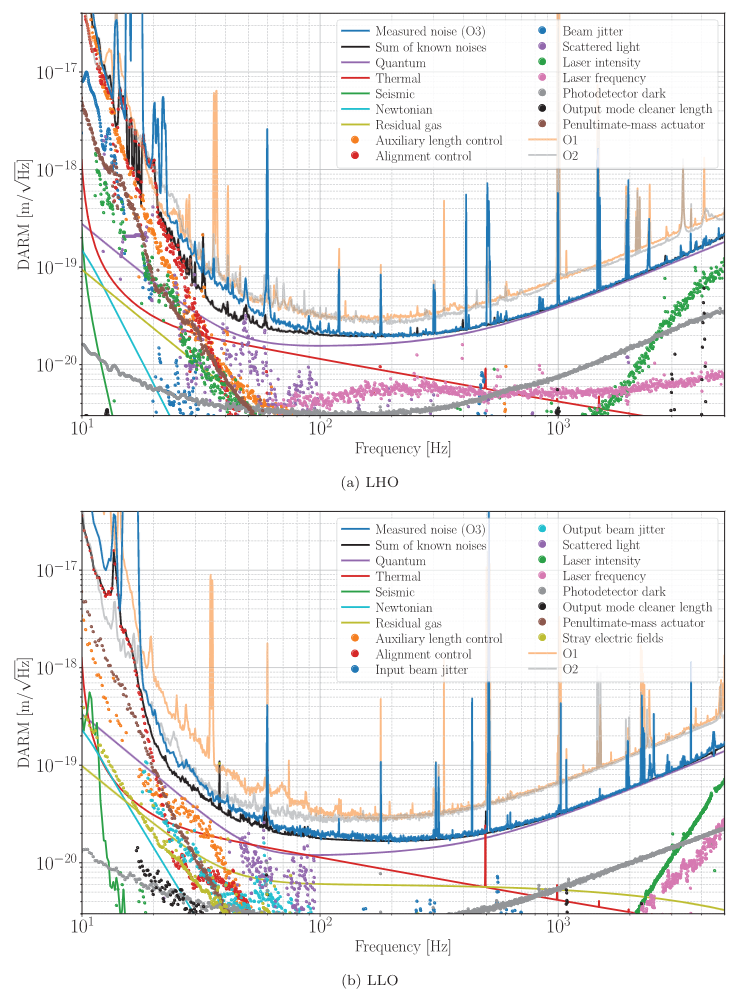
\includegraphics[width=0.6\linewidth]{sectionDetection/ligo_sensitivity_screenshot.png}
%   \caption{Contributions de différentes sources de bruit aux ASD des détecteurs LIGO Livingston et Hanford durant O3. Figure issue de \cite{ligo_sensitivity}.}
%   \label{fig:ligo_sensitivity}
% \end{figure}

\begin{figure}
  \centering
  \begin{minipage}{\linewidth}
    \centering
    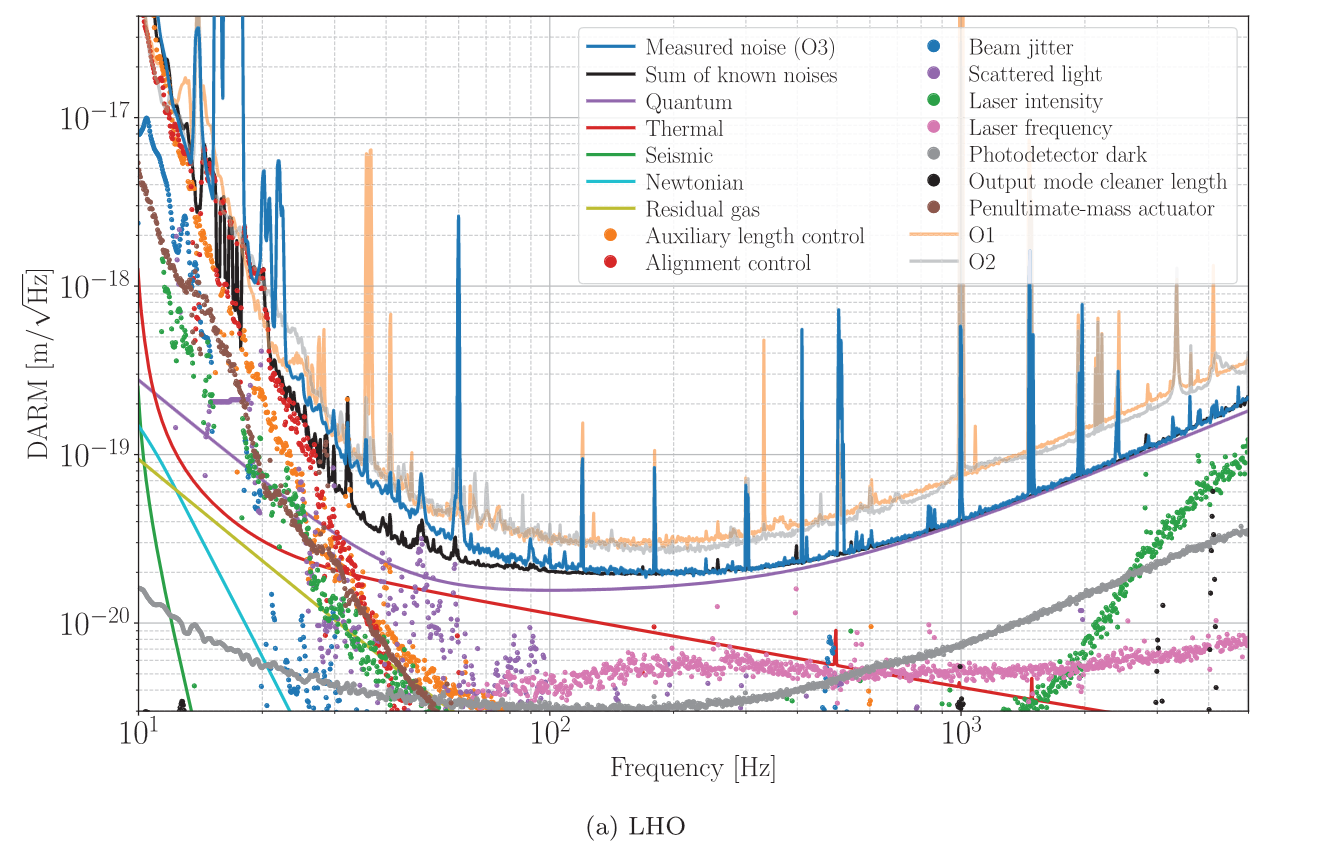
\includegraphics[width=\linewidth]{sectionDetection/ligo_sensitivity_lho.png}
  \end{minipage}
  %
  \begin{minipage}{\linewidth}
    \centering
    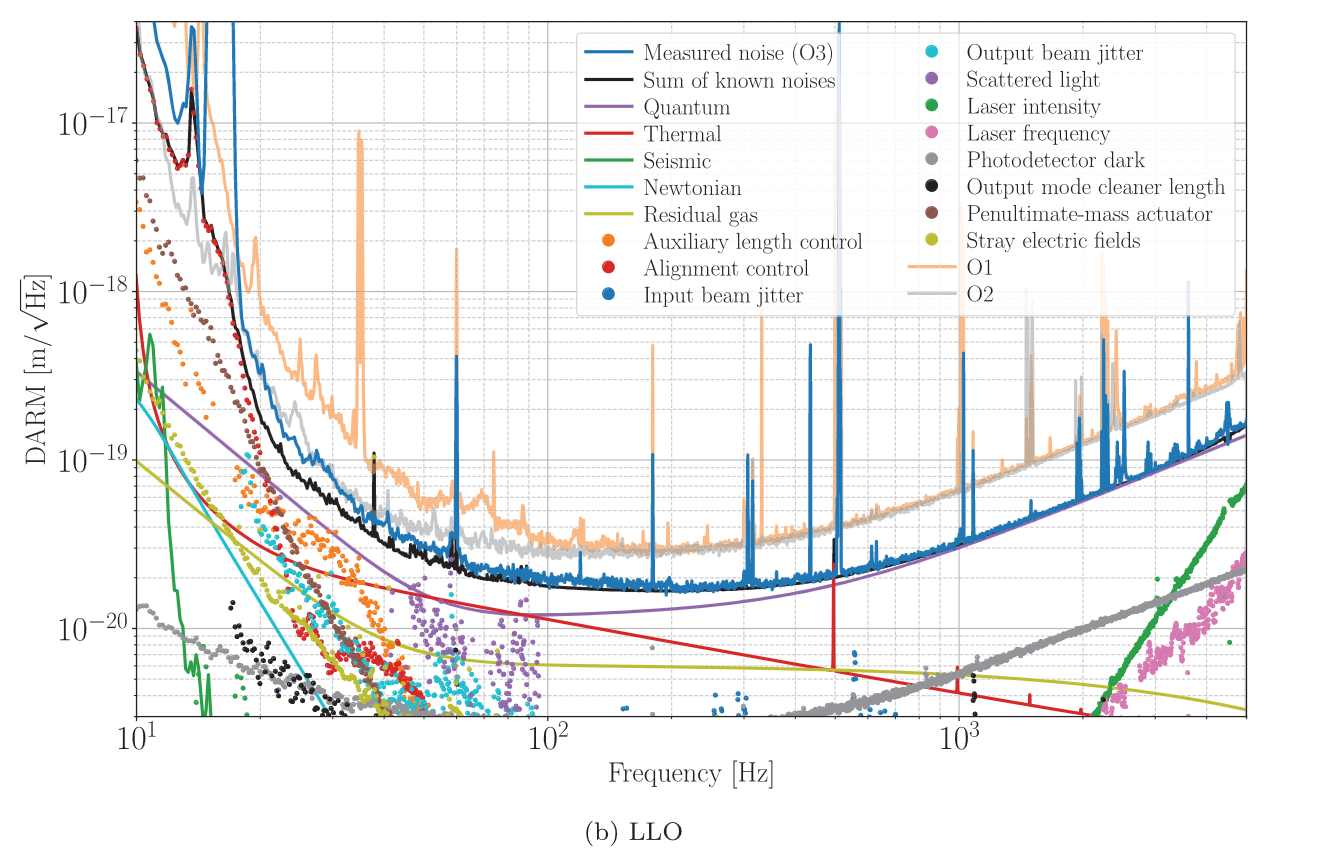
\includegraphics[width=\linewidth]{sectionDetection/ligo_sensitivity_llo.png}
  \end{minipage}
  \caption{Contributions de différentes sources de bruit aux ASD des détecteurs LIGO Livingston et Hanford durant O3. Figure issue de \cite{ligo_sensitivity}.}
  \label{fig:ligo_sensitivity}
\end{figure}


\begin{figure}
  \centering
  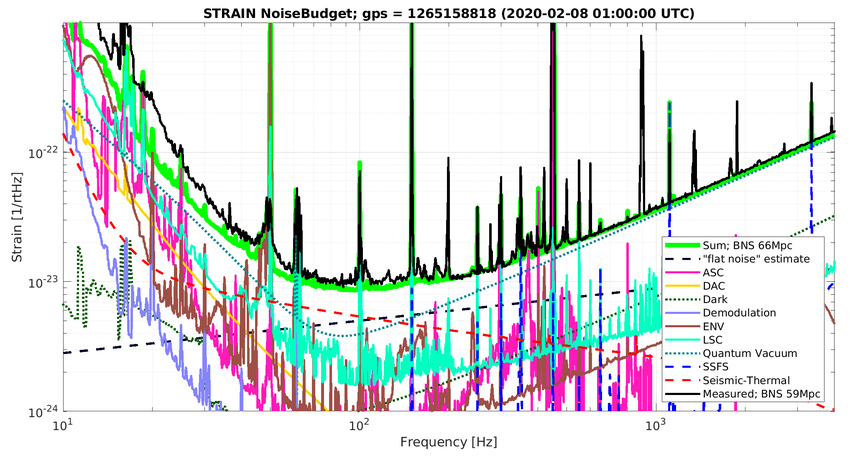
\includegraphics[width=0.7\linewidth]{sectionDetection/virgo_noise.png}
  \caption{Contributions de différentes sources de bruit à l'ASD du détecteur Virgo pendant O3. Figure issue de \cite{virgo_characterization}.}
  \label{fig:virgo_sensitivity}
\end{figure}


\begin{figure}
  \centering
  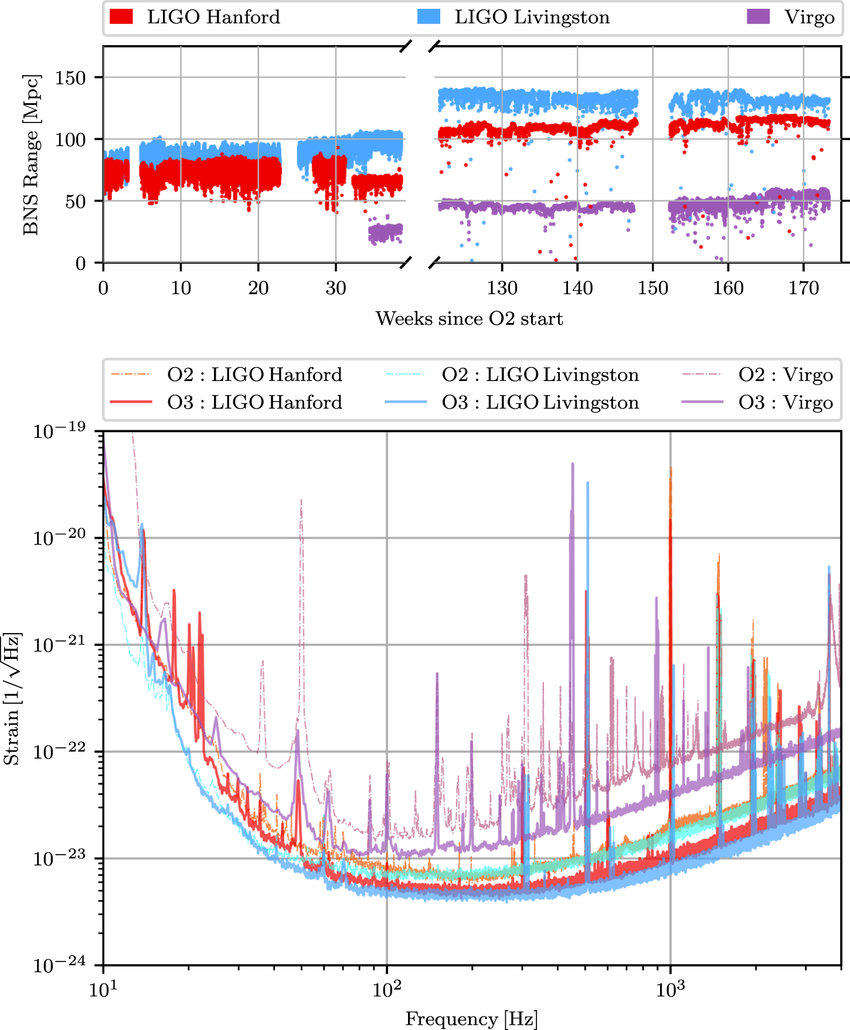
\includegraphics[width=0.6\linewidth]{sectionDetection/sensitivity_comparison.png}
  \caption{Comparaison des sensibilités de O3 et O2 pour les détecteurs LIGO et Virgo \cite{ligo_characterization}.}
  \label{fig:sensitivity_comparison}
\end{figure}


\begin{figure}
  \centering
  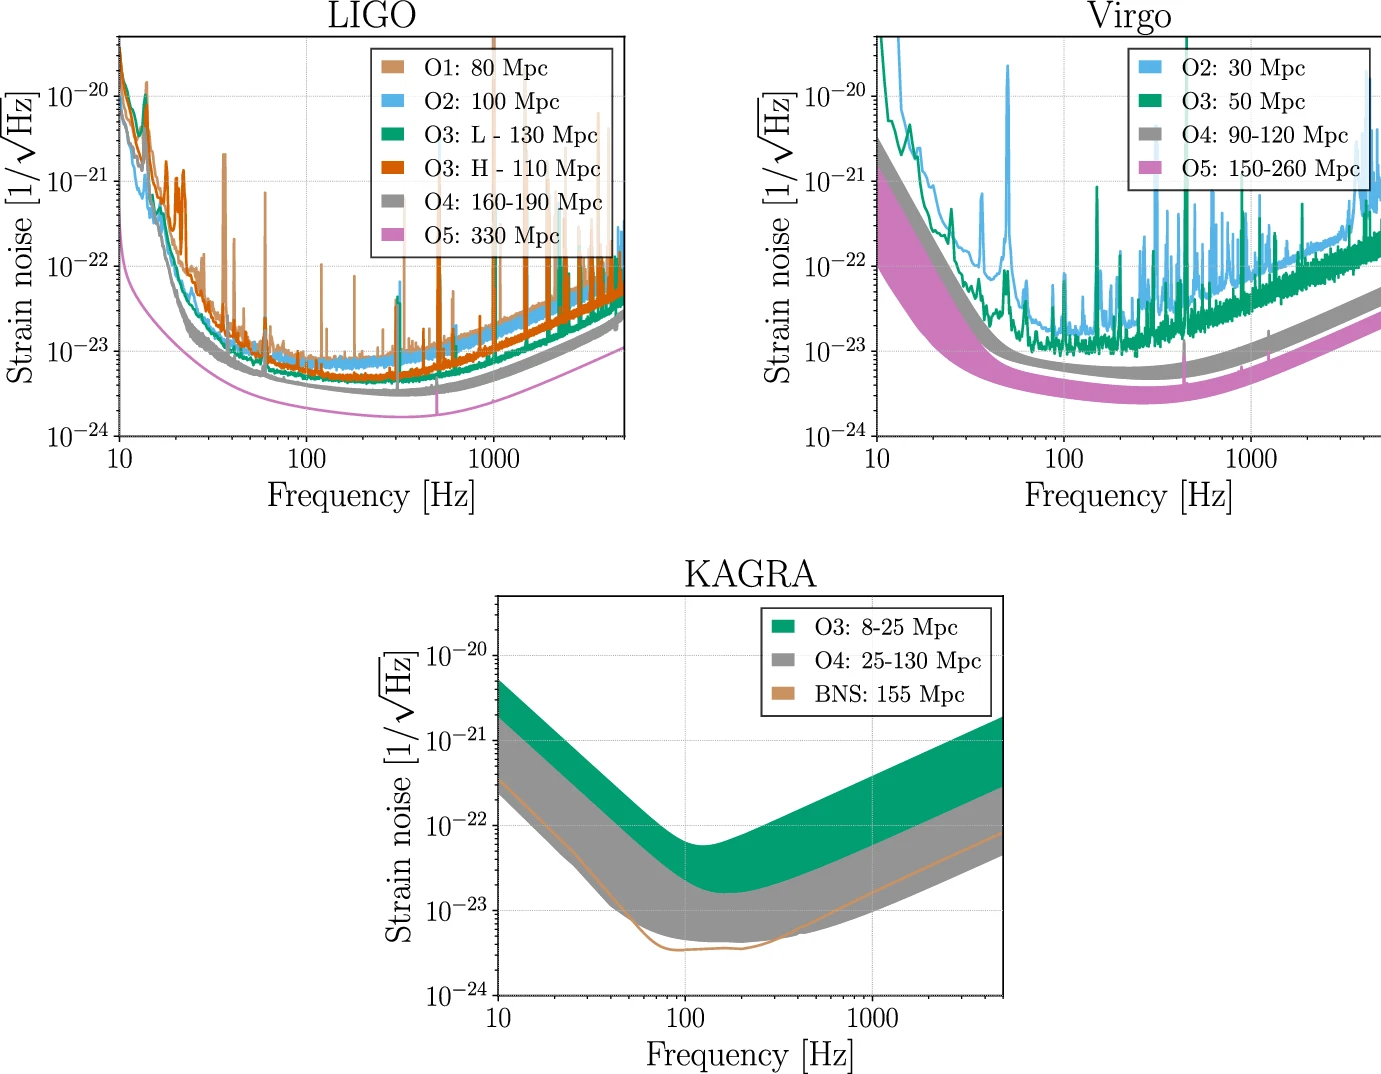
\includegraphics[width=\linewidth]{sectionDetection/design_sensitivities.png}
  \caption{Evolution des sensibilités pour les détecteurs LIGO, Virgo et KAGRA \cite{prospects}.}
  \label{fig:design_sensitivities}
\end{figure}



%%%%%%%%%%
\clearpage \newpage
\subsection{Réseau de détecteur et localisation des sources}
\label{sec:network}

Pendant O3, trois détecteurs d'ondes gravitationnelles ont été utilisé pour faire des détections: LIGO Hanford (H1, USA), LIGO Livingston (L1, USA) et Virgo (V1, Italie).
Le détecteur GEO600 (Allemagne) observe le ciel depuis plusieurs années.
Il est principalement utilisé pour faire de la recherche et du développement d'équipements dédiés aux autres détecteurs.
Le détecteur KAGRA (Japon) a effectué une courte période d'observation à la fin de O3.
Un troisième détecteur LIGO est également prévu en Inde.
La figure \ref{fig:igwn} montre ce réseau d'interféromètre sur un planisphère.
%
\begin{figure}
  \centering
  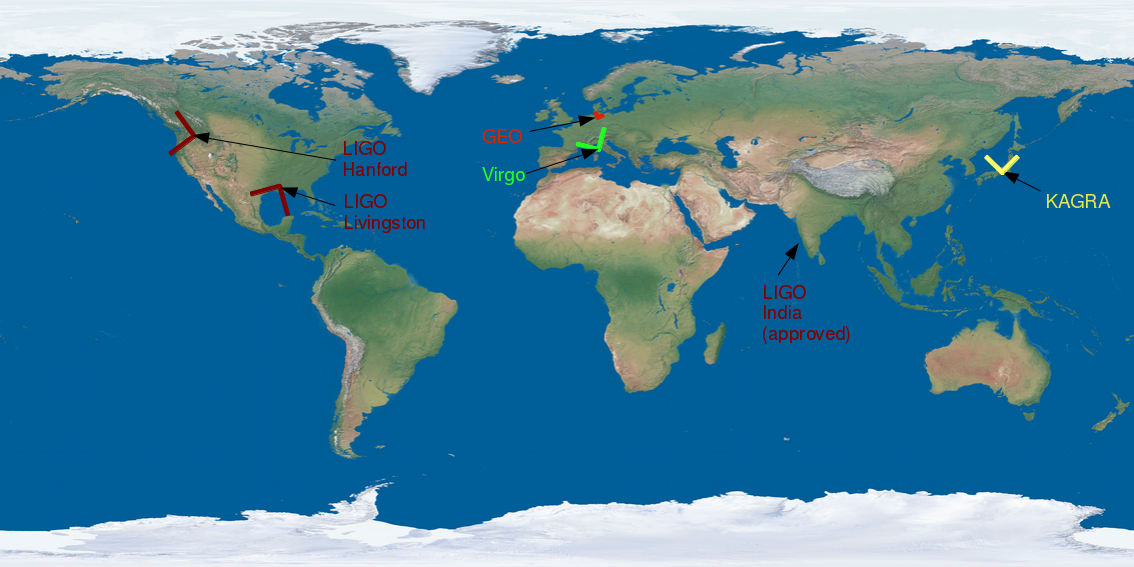
\includegraphics[width=0.8\linewidth]{sectionDetection/itf_network.png}
  \caption{Carte du réseau international d'observatoires d'ondes gravitationnelles (IGWN) indiquant également l'orientation des détecteurs. Issue de \href{http://public.virgo-gw.eu/a-worldwide-network/}{site web Virgo}.}
  \label{fig:igwn}
\end{figure}
%

Il y a de multiples bénéfices à avoir plusieurs détecteurs.
Tout d'abord, en les plaçant à des positions différentes sur Terre avec des orientations également différentes, les diagrammes d'antennes des détecteurs vont se compléter.
Cela permet d'avoir une bien meilleure couverture du ciel et d'augmenter les chances de détection.

Un autre avantage est la possibilité de rechercher des signaux en coïncidence dans plusieurs détecteurs.
Dans le cas de la recherche de CBC, nous pouvons en effet supposer que le bruit des différents détecteurs n'est pas corrélé car il ne dépend que de facteurs locaux (nous ne considérons aucune source de bruit astrophysique) et les détecteurs sont largement séparés.
Ainsi, un signal fort causé par du bruit dans un détecteur a très peu de chances d'être associé à un signal fort causé par du bruit dans un autre détecteur au même moment.
Par contre, dans le cas d'évènements astrophysiques, les ondes traversent la Terre et tous les détecteurs sont susceptible de les détecter.
Dans ce cas on s'attend à avoir des signaux significatifs similaires dans plusieurs détecteurs à la fois (en prenant en compte le temps de vol des ondes entre les détecteurs).
C'est un critère puissant qui permet de discriminer signaux astrophysiques et bruit de fond.

Un troisième bénéfice, qui est en fait le produit des deux considération précédentes, est qu'un plus grand nombre de détecteurs permet d'avoir une meilleure localisation de la source des ondes.
Pour une amplitude relative et un delai de détection entre des détecteurs, il est possible de trianguler la position la plus probable pour la source des ondes gravitationnelles.
La non-détection d'un signal par l'un des détecteurs est également une information intéressante car cela indique que la source peut être localisée dans une direction à laquelle ce détecteur n'est pas sensible.
Le processus de localisation est illustré en figure \ref{fig:localization} en prenant l'exemple de GW170817.
De gauche à droite et de haut en bas: les réponses d'antennes de H1 et L1 indiquent les directions auxquelles ils sont sensibles.
L'information temporelle permet de définir une ligne sur le ciel sur laquelle il est probable que la source soit positionnée.
En prenant en compte les rapports d'amplitude dans H1 et L1 il est possible de dériver un contour pour la position de la source autour de cette ligne.
Si on ajoute maintenant V1, qui n'a pas détecté l'évènement, on peut raffiner la recherche de la position.
Comparer les SNR mesurés aux SNR attendus en fonction de la position de la source  permet également d'inférer un contour plus restreint pour la position de la source.

\begin{figure}
  %
  % 1
  \begin{minipage}{0.45\linewidth}
    \centering
    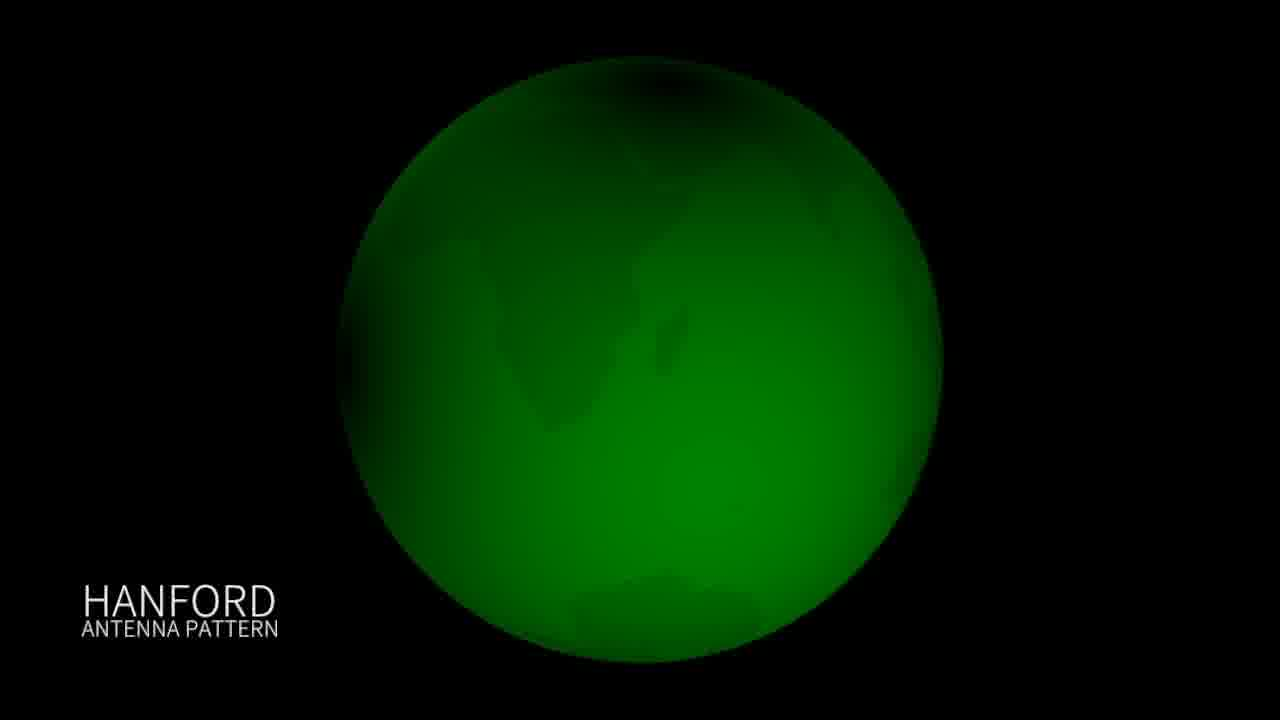
\includegraphics[width=\linewidth]{sectionDetection/antenna-patterns_LeoSinger/00012.jpg}
    %\captionof*{figure}{(a) LIGO Hanford antenna pattern, the dark areas are the less sensitive ones.}
  \end{minipage}
  %
  \hfill
  % 2
  \begin{minipage}{0.45\linewidth}
    \centering
    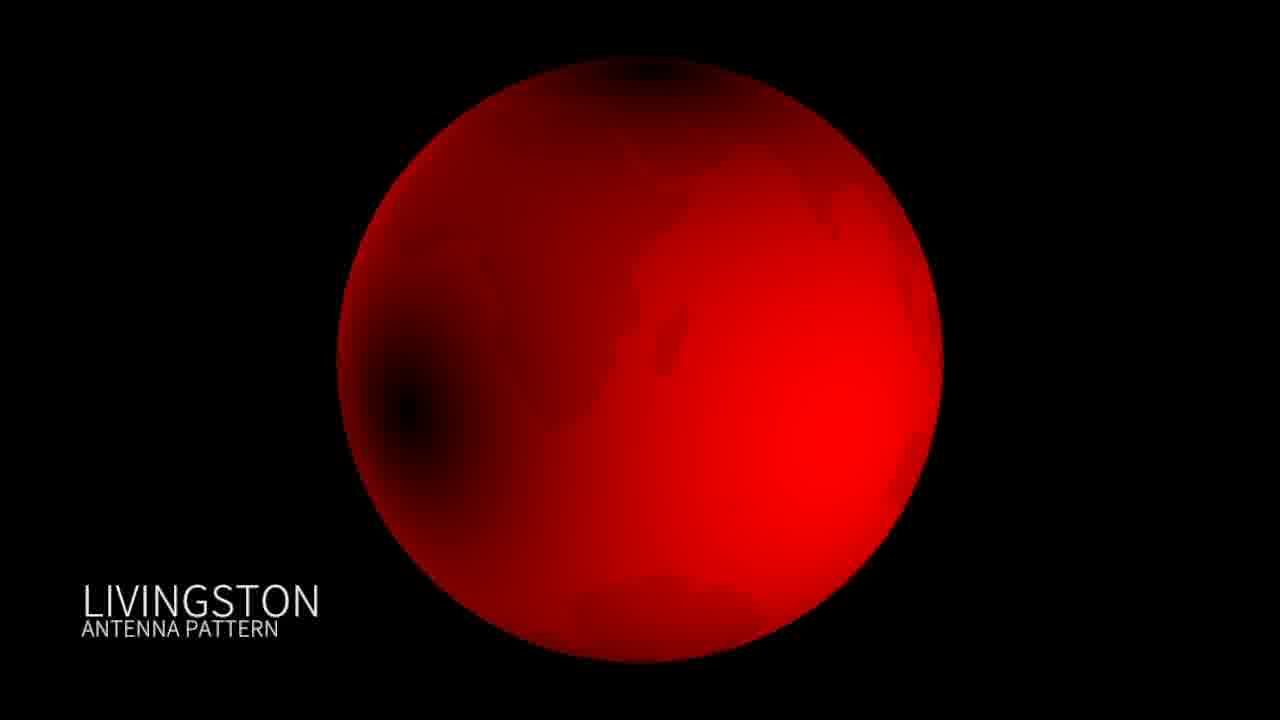
\includegraphics[width=\linewidth]{sectionDetection/antenna-patterns_LeoSinger/00118.jpg}
    %\captionof*{figure}{(b) LIGO Livingston antenna pattern, the dark areas are the less sensitive ones.}
  \end{minipage}
  %
  \hfill
  % 3
  \begin{minipage}{0.45\linewidth}
    \centering
    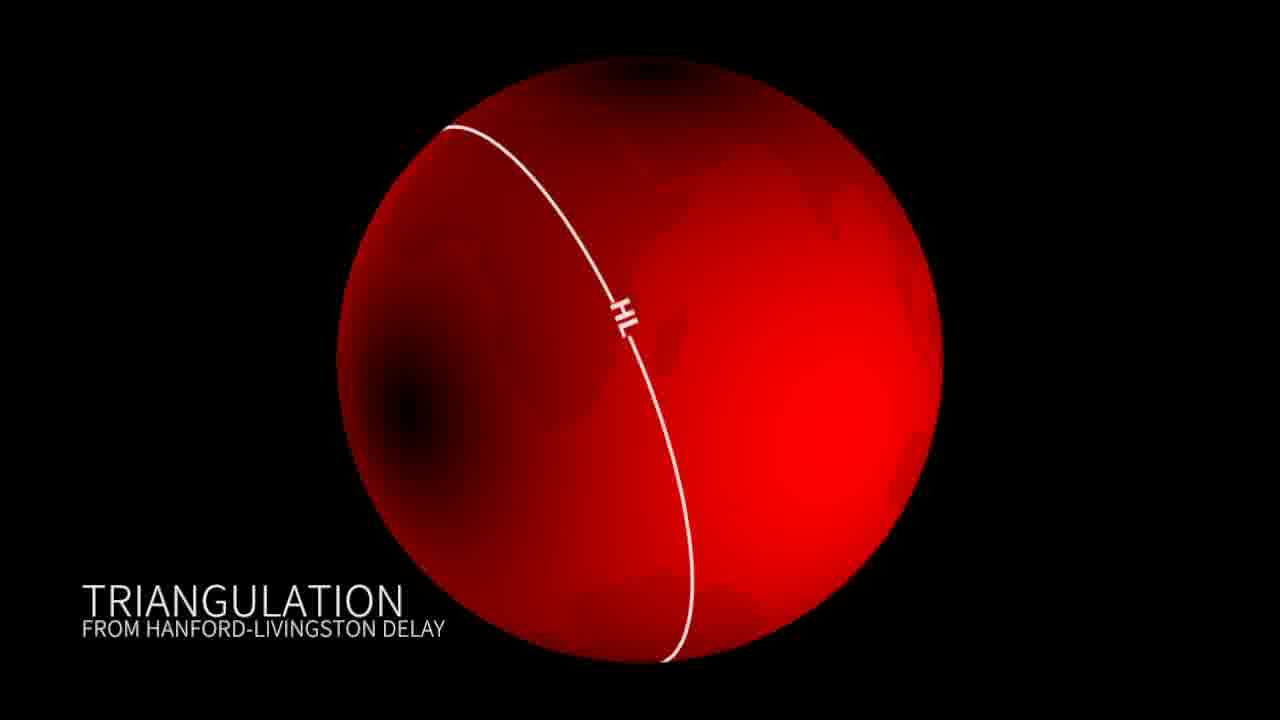
\includegraphics[width=\linewidth]{sectionDetection/antenna-patterns_LeoSinger/00227.jpg}
    %\captionof*{figure}{(c) Line of sight given by the timing information between H1 and L1.}
  \end{minipage}
  %
  \hfill
  % 4
  \begin{minipage}{0.45\linewidth}
    \centering
    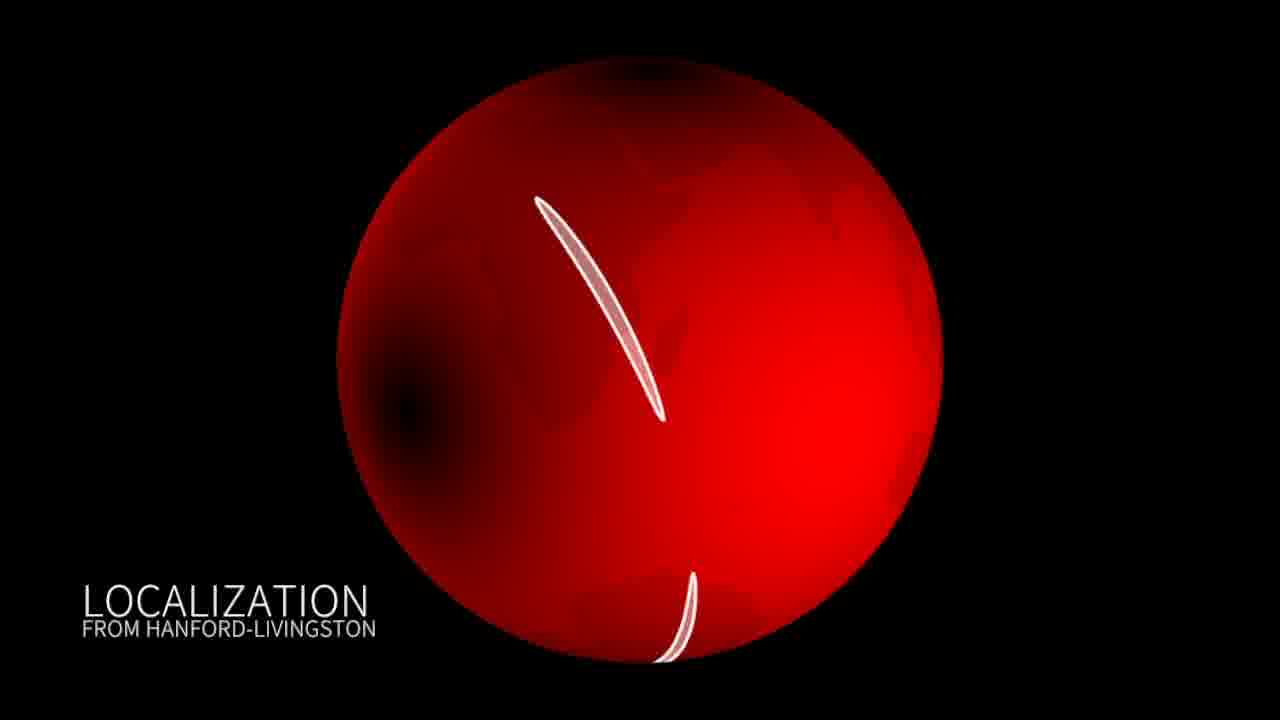
\includegraphics[width=\linewidth]{sectionDetection/antenna-patterns_LeoSinger/00318.jpg}
    %\captionof*{figure}{(d) Source localization contour obtained by accounting for the SNR in H1 and L1.}
  \end{minipage}
  %
  \hfill
  % 5
  \begin{minipage}{0.45\linewidth}
    \centering
    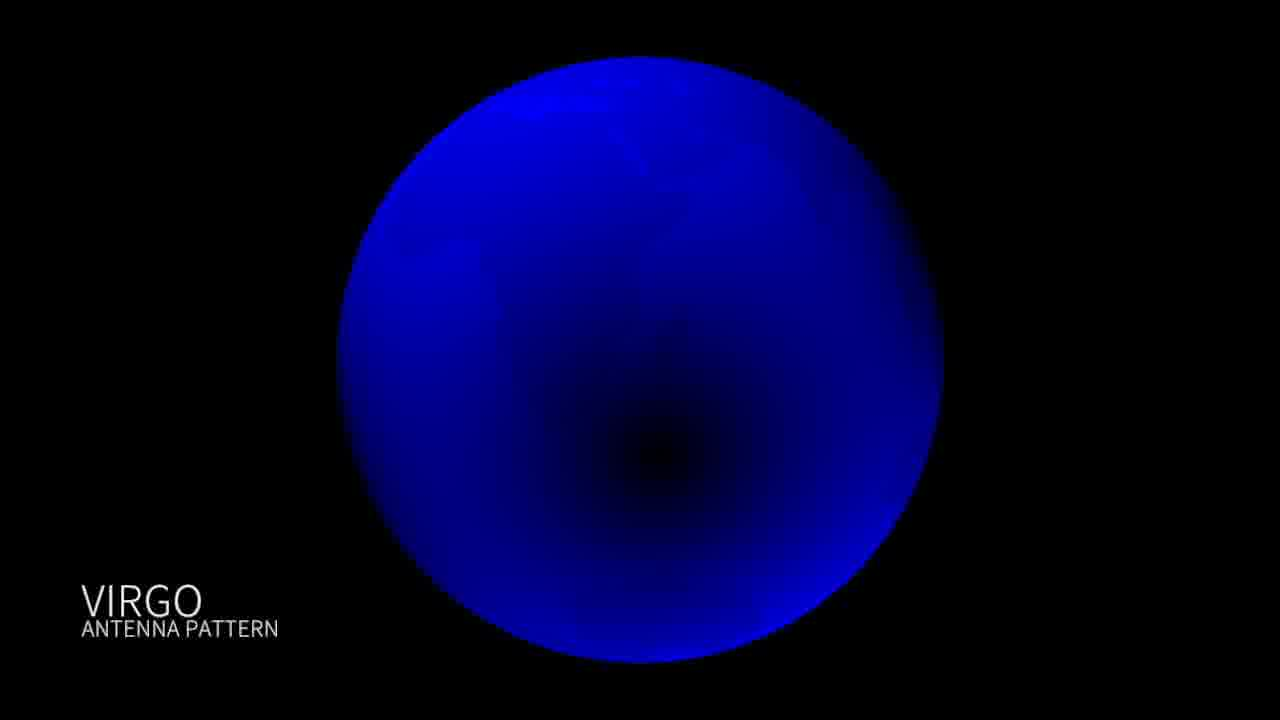
\includegraphics[width=\linewidth]{sectionDetection/antenna-patterns_LeoSinger/00418.jpg}
    %\captionof*{figure}{(e) Virgo antenna pattern, the dark areas are the less sensitive ones.}
  \end{minipage}
  %
  \hfill
  % 6
  \begin{minipage}{0.45\linewidth}
    \centering
    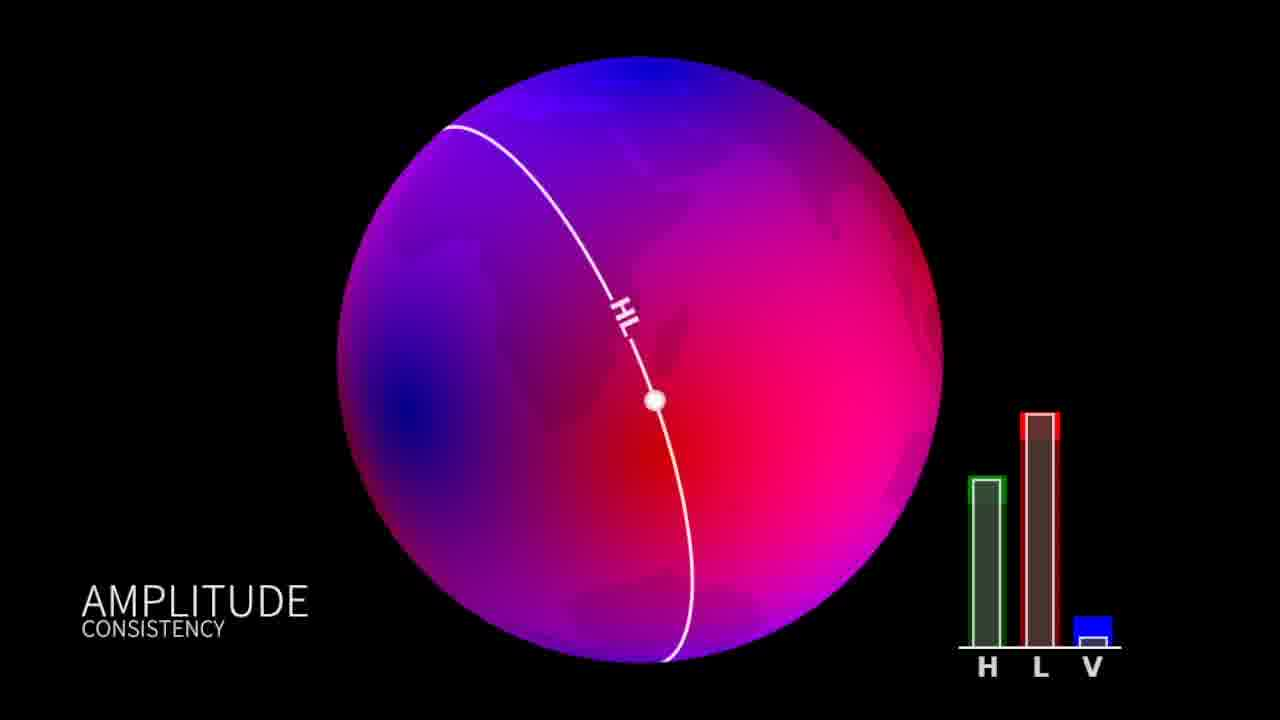
\includegraphics[width=\linewidth]{sectionDetection/antenna-patterns_LeoSinger/00552.jpg}
    %\captionof*{figure}{(f) Attempt at finding the source localization by estimating the expected SNRs int the three detectors.}
  \end{minipage}
  %
  \hfill
  % 7
  \begin{minipage}{0.45\linewidth}
    \centering
    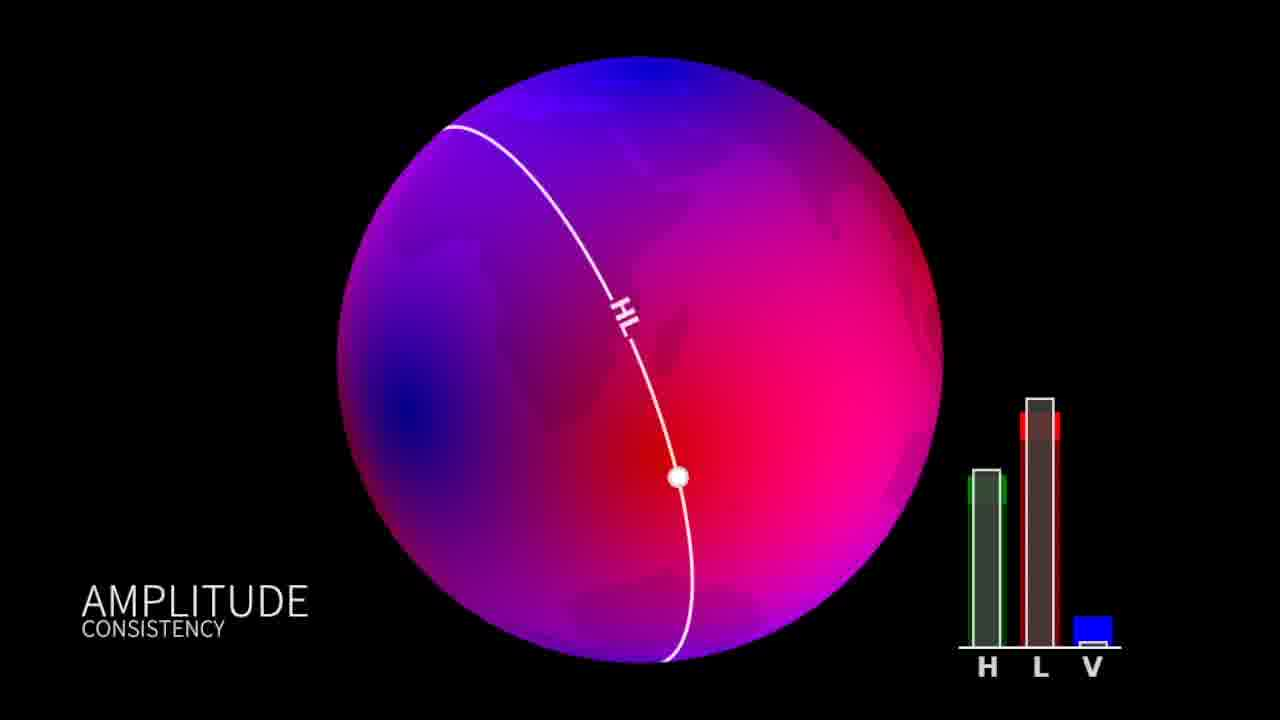
\includegraphics[width=\linewidth]{sectionDetection/antenna-patterns_LeoSinger/00559.jpg}
    %\captionof*{figure}{(g) Attempt at finding the source localization by estimating the expected SNRs int the three detectors.}
  \end{minipage}
  %
  \hfill
  % 8
  \begin{minipage}{0.45\linewidth}
    \centering
    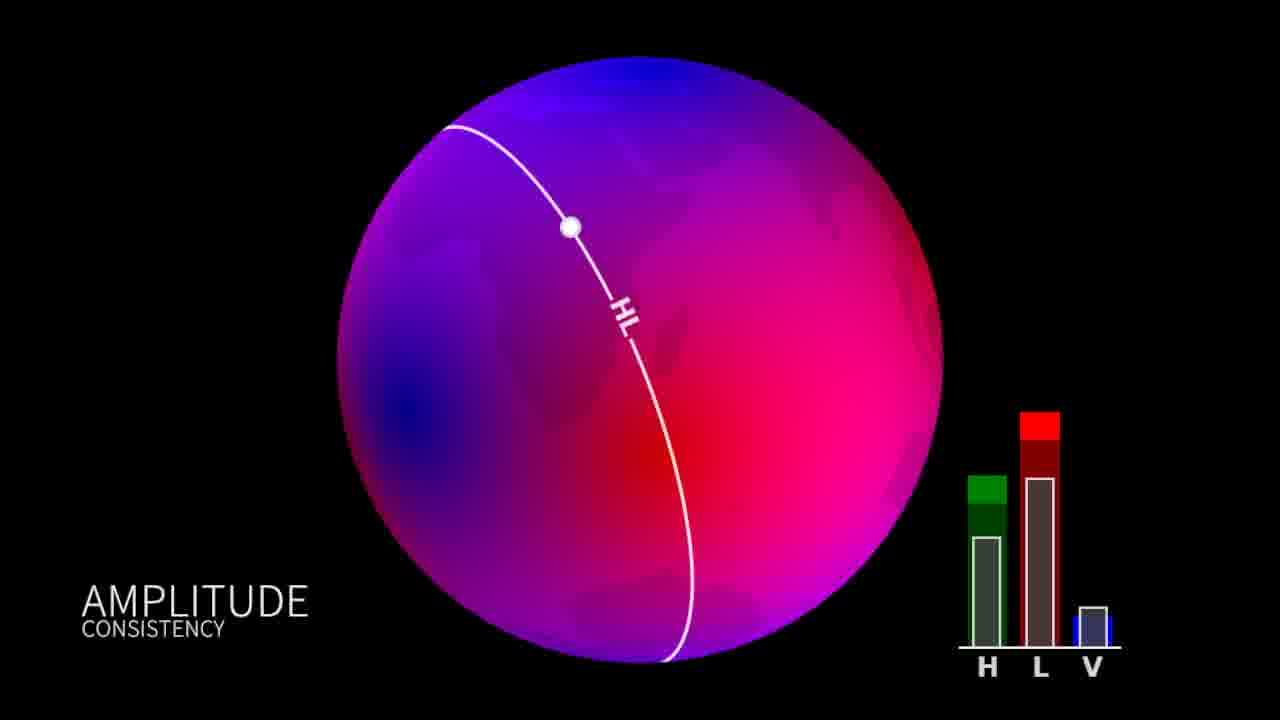
\includegraphics[width=\linewidth]{sectionDetection/antenna-patterns_LeoSinger/00584.jpg}
    %\captionof*{figure}{(h) Attempt at finding the source localization by estimating the expected SNRs int the three detectors.}
  \end{minipage}
  %
  \hfill
  % 9
  \centering
  \begin{minipage}{0.45\linewidth}
    \centering
    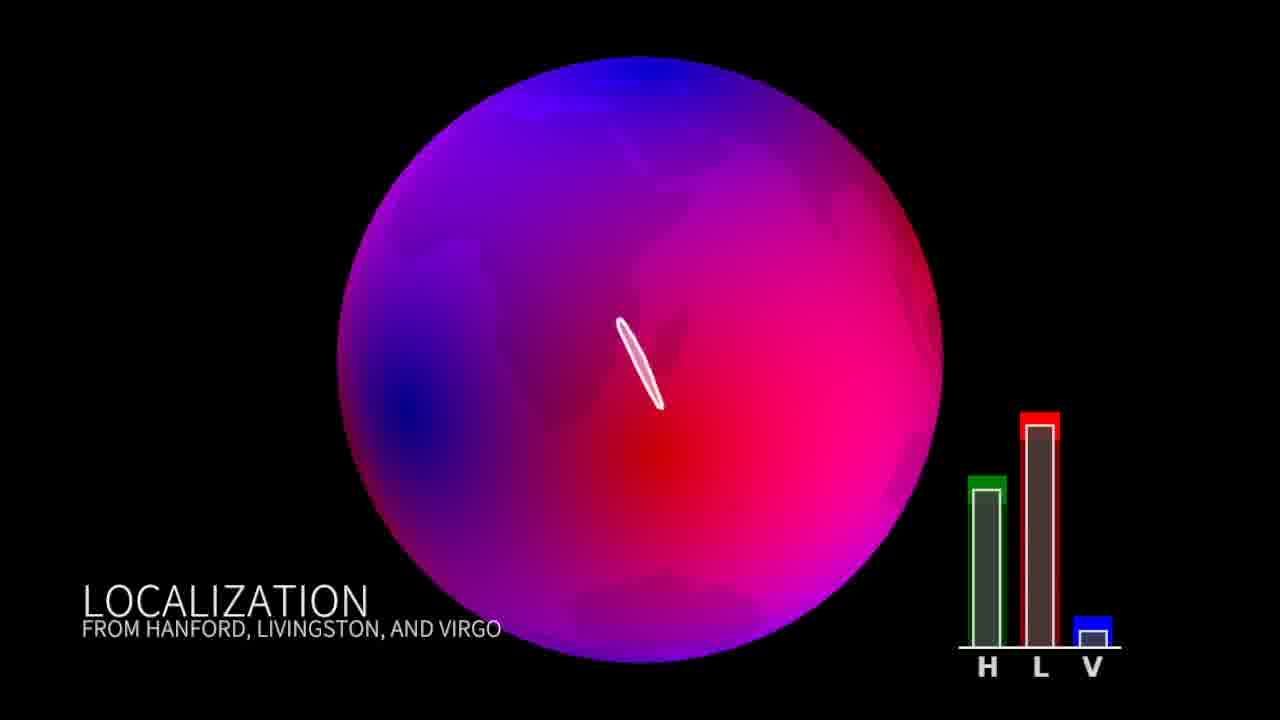
\includegraphics[width=\linewidth]{sectionDetection/antenna-patterns_LeoSinger/00900.jpg}
    %\captionof*{figure}{(i) Refined source localization contour obtained by including V1.}
  \end{minipage}
  %
  \hfill
  \caption{Illustration du processus de localisation d'une source d'ondes gravitationnelles, appliquée à GW170817. Voir le texte pour une description. Crédit: Leo Singer (format original disponible à \url{https://dcc.ligo.org/LIGO-G1702012/public}).}
  \label{fig:localization}
\end{figure}


%%%%%%%%%%
\subsection{Publication d'alertes en ligne}
Dans le cas de GW170817, une information supplémentaire était disponible pour localiser la source.
En effet, une contrepartie électromagnétique fut détectée.
La figure \ref{fig:gw170817_location} résume les informations données par les divers observatoires.
%
\begin{figure}
  \centering
  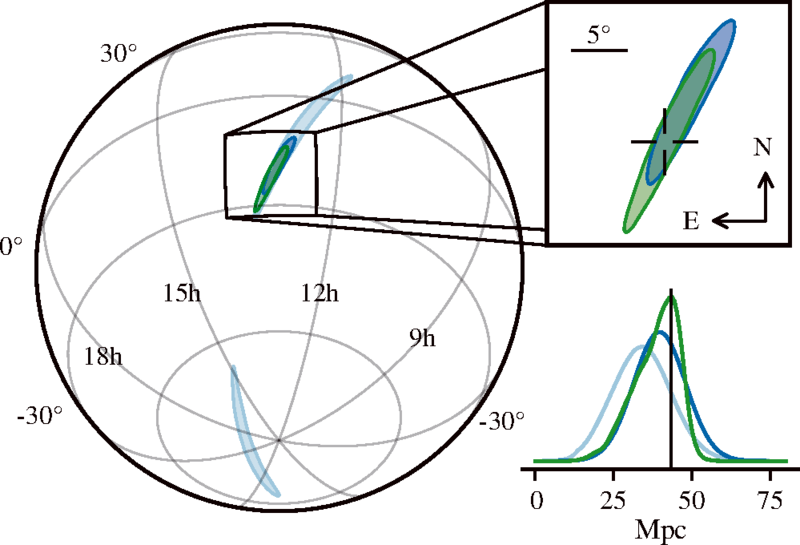
\includegraphics[width=0.5\linewidth]{sectionDetection/gw170817_location.png}
  \caption{Reconstruction de la position de la source dans le ciel pour GW170817 issue de \cite{gw170817}.
    L'aire bleu-clair (190 deg$^2$) est calculée par un algorithme de réponse rapide en n'utilisant que H1 et L1.
    La bleu-foncé (31 deg$^2$) inclut V1.
    Le contour vert (28 deg$^2$) inclut les trois détecteurs, il est donné par un algorithme avec une latence plus élevée que le précédent.
    Le réticule dans le paneau en haut à droite indique la position de la galaxie hôte identifiée.
    Le paneau en bas à droite donne la distribution postérieure pour la distance de luminosité.}
  \label{fig:gw170817_location}
\end{figure}
%
Cette détection conjointe est rendue possible grâce au systeme d'alertes publiques émisent par la collaboration LVK et utilisée par de nombreux observatoires dans le monde.

Les chaînes d'analyse utilisent un seuil de taux de fausse alarme (FAR), typiquement de l'ordre de un par deux heures, pour envoyer leurs candidats à la base de donnée commune GraceDB.
Le FAR est le taux d'évènements de bruit de fond que l'on attend avec une statistique de classement supérieure à un seuil donné.
Les candidats enregistrés par GraceDB sont rangés dans des structures appelées ``G-event''  avec certaines propriétés rapportées par la chaîne d'analyse.
Si plusieurs chaînes ont détecté un même évènement, un ``Superevent'' est créé et rassemble les différents G-events associés à la détection.
Les propriétés listées dans le superevent sont celles du G-event dit ``préféré'', choisi comme celui ayant le plus grand SNR.
Les notices contiennent de nombreux paramètres comme le type et le temps de l'alerte, la chaîne d'analyse qui a rapporté la détection, les détecteurs impliqués, la carte du ciel et les diverses probabilités cité plus bas dans cette section.

Le FAR des candidats est utilisé pour définir leur significativité.
Lorsque le FAR d'un candidat rapporté par au moins l'une des chaînes d'analyse dépasse un certain seuil, fixé par la collaboration, le candidat est rendu public (au-delà de la collaboration LVK) et des circulaires et notices sont envoyées aux observatoires qui en ont fait la demande.
Plusieurs chaînes d'analyse CBC (MBTA, PyCBC, GstLAL, SPIIR, cWB\_BBH, RAVEN) peuvent participer aux détections.
Pour prendre en compte cette multiplicité, le bruit qu'elles détectent est supposé indépendant et donc les seuils par chaîne d'analyse valent le seuil global divisé par le nombre de chaînes d'analyses CBC.
On parle de ``\textit{trial factor}''.

Durant O3 le seuil de FAR global était défini comme un tous les deux mois pour les candidats CBC.
Comme il y avait cinq chaînes d'analyse CBC, le seuil par chaîne d'analyse était donc de un tous les dix mois.

Pour O4 deux seuils globaux sont considérés:
\begin{itemize}
\item FAR$<$1 par mois pour les candidats significatifs,
\item 1 par mois$<$FAR$<$2 par jour pour les candidats faiblement significatifs.
\end{itemize}
Cela donne respectivement, pour les FAR calculés par les chaines d'analyse, des seuils à 1 par 6 mois et 1 par trois jours après application du \textit{trial factor}.
%
Le seuil pour les recherches de bursts est quant à lui de 1 par an avec un \textit{trial factor} de 1/3 pour prendre en compte les trois chaînes d'analyse.
Les candidats significatifs sont validés par les experts des chaînes d'analyse et de la caractérisation des détecteurs ayant participés à la détection sous la forme d'une circulaire.
Cela permet de confirmer le potentiel de l'évènement ou bien de retirer l'alerte si un expert juge que l'évènement n'est pas d'origine astrophysique.

Pour O4 une catégorie supplémentaire d'évènements existe: les candidats dits de ``haut profil'' auxquels une attention particulière est portée.
Il s'agit de candidats significatifs qui satisfont l'une des conditions suivantes:
\begin{itemize}
\item Une contrepartie multi-messager a été détectée,
\item Le G-event avec le plus faible FAR a été téléchargé par une chaîne d'analyse de burst,
\item Le G-event préféré a une probabilité d'origine astrophysique (voir section \ref{sec:pastro} pour une définition de ces quantités) supérieure à 0.5 et:
  \begin{itemize}
  \item soit la probabilité qu'il s'agisse d'une BNS est supérieure à 10\%,
  \item soit la probabilité qu'il s'agisse d'une NSBH est supérieure à 10\%,
  \item soit la probabilité qu'il y ait une masse résiduelle après la fusion est supérieure à 10\%,
  \item ou bien le contour à 90\% de niveau de confiance pour la position de la source est plus petit que 100 deg$^2$.
  \end{itemize}
\end{itemize}

Plus d'informations sur le système d'alertes peuvent être trouvées dans le guide d'utilisateur fourni par la collaboration LVK: \url{https://emfollow.docs.ligo.org/userguide/}.

%%%%%%%%%%
\clearpage\newpage
\subsection{Autres détecteurs d'ondes gravitationnelles}
%describe shortly ET, LISA, Cosmic Explorer

D'autres détecteurs d'ondes gravitationnelles sont proposés avec des stades de progression plus ou moins avancés.
Leur modèles peuvent donc encore être amenés à changer.

\subsubsection*{Détecteurs de troisième génération}

Le ``Einstein Telescope'' (ET) \cite{ET} est une proposition d'interféromètre sous-terrain dix fois plus sensible que les détecteurs de seconde génération LIGOs et Virgo.
Deux propositions ont été formulées concernant sa forme: triangulaire ou en forme de L (à l'instar des LIGOs/Virgo) avec des bras bien plus grand que les détecteurs acutels.
Deux sites sont pour le moment considérés: la Sardaigne et l'Euroregio Meuse-Rhin.

Cosmic Explorer (CE) est une proposition de détecteur aux USA.
Il est prévu en forme de L avec des bras de \SI{40}{km} et une sensibilité dix fois plus grande que les détecteurs Advanced LIGO.

ET et CE permettraient des mesures extrêmement précises des paramètres des sources, ce qui contraindrait de nombreux modèles.
Il y a également des attentes concernant la première détection directe de bruit de fond stochastique d'ondes gravitationnelles et un raffinement des mesures de LIGO et Virgo.

\subsubsection*{LISA}
Le ``Laser Interferometer Space Antenna'' (LISA) \cite{LISA} est une proposition d'observatoire basé dans l'espace.
Son but serait d'étudier les basses fréquences entre \SI{0.1}{\milli\hertz}$-$\SI{0.1}{\hertz}.
Son design consiste en trois satellites formant un triangle.
Chacun abrite deux masses libres et deux lasers qu'ils pointent vers leurs voisins.
Les satellites seraient séparés d'environ $\sim 2.5$ million \si{km}.
Les variations relatives de distance entre les masses libres situées dans les satellites sont mesurées par interférométrie laser hétérodyne.


\subsubsection*{Pulsar Timing Array}
Le réseau de synchronisation de pulsar international, ou \textit{International Pulsar Timing Array} (IPTA), est un détecteur d'ondes gravitationnelles ``naturel'' exploitant les émissions périodiques de pulsars connus \cite{IPTA}.
Le passage d'une onde gravitationnelle causera un delai dans le temps de vol des impulsions émises par les pulsars, corrélées avec la position dans le ciel de ces derniers permettant la détection.
L'éloignement des pulsars étant bien plus grand que les bras des détecteurs terrestres, IPTA pourra sonder des fréquences très faibles allant jusqu'au nanoHertz.

La collaboration NANOGrav, membre du consortium IPTA a récemment publié des premières observations de l'existence d'un bruit de fond stochastique d'ondes gravitationnelles \cite{nanograv}.
Une corrélation entre 67 pulsars a été observée en utilisant 15 ans de données collectées par NANOGrav.
Cette corrélation suit le modèle de Hellings-Downs, attendu pour un signal stochastique d'ondes gravitationnelles.
Le spectre et l'amplitude observés correspondent aux attentes pour une population de binaires de trous noirs supermassifs.